\documentclass[12pt]{article}
\usepackage[utf8]{inputenc}
\usepackage{amsfonts}
\usepackage{amsmath}
\usepackage{graphicx}
\usepackage{fullpage}
\usepackage{subcaption}
\usepackage{float}

\title{Projet COMPLEX\\Problème du VERTEX COVER}
\author{Esther CHOI (3800370)\\Folco BERTINI (3802296)\\M1 DAC - Groupe 1}

\begin{document}

\maketitle
\tableofcontents

\begin{abstract}
    Ce document constitue le rapport du projet de l'UE COMPLEX, suivie au premier semestre du M1 Informatique à Sorbonne Université. \\
    Les tests de performance des différents algorithmes ont été réalisés avec un processeur AMD Ryzen 7 3700X 8-Core 1.87 GHz. \\
\end{abstract}

\newpage

\section{Définition du problème}

    Une couverture d'un graphe est un ensemble de sommets qui couvre toutes les arêtes du graphe (une arête est couverte lorsqu'au moins une de ses extrémités se trouve dans la couverture). \\
    Le problème \textsc{vertex cover} est défini de la façon suivante :

    \begin{itemize}
        \item entrée : un graphe non orienté G
        \item sortie : une couverture de G de taille minimale
    \end{itemize}

    Le but de ce projet est d'implémenter des algorithmes approchés et exacts pour résoudre le problème \textsc{vertex cover}.

\section{Graphes}

    Pour l'implémentation de nos graphes, nous avons choisi d'utiliser la librairie \texttt{networkx} qui contient de nombreuses fonctions pratiques dont nous nous sommes servies pour coder les méthodes de base.
    
\section{Méthodes approchées}

    \paragraph{3.1)}
        Soit le graphe $I$ suivant :

        \begin{figure}[h]
            \caption{Graphe $I$}
            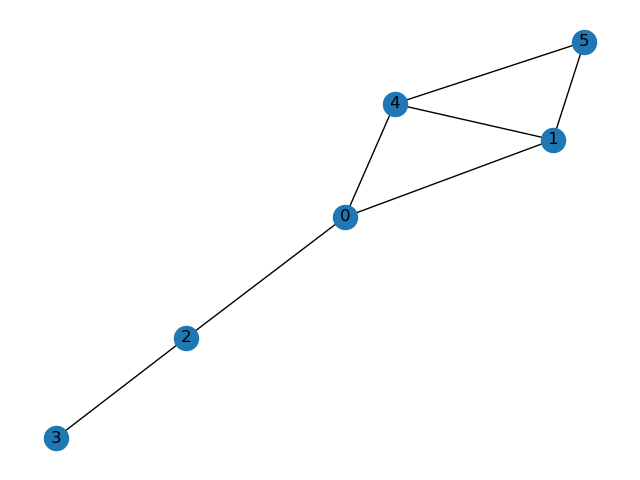
\includegraphics[scale=0.6]{figures/q3-1.png}
            \centering
        \end{figure}

        Une couverture optimale est $C_{opt} = \{1,2,4\}$. L'algorithme glouton renvoie la solution $C = \{0,1,2,4\}$ qui a un sommet de plus. \\
        En effet, voici l'exécution complète de \texttt{algo\_glouton} pour ce graphe $I$ :

        \begin{itemize}
            \item initialisation : arêtes $E = [\{0,2\},\{0,1\},\{0,4\},\{1,4\},\{1,5\},\{2,3\},\{4,5\}]$ \\
            couverture $C = \{\}$
            \item boucle while :
                \begin{itemize}
                    \item $C = \{0\}$ \\
                    $E = [\{1,4\},\{1,5\},\{2,3\},\{4,5\}]$
                    \item $C = \{0,1\}$ \\
                    $E = [\{2,3\},\{4,5\}]$
                    \item $C = \{0,1,2\}$ \\
                    $E = [\{4,5\}]$
                    \item $C = \{0,1,2,4\}$ \\
                    $E = []$
                \end{itemize}
            \item résultat final : $C = \{0,1,2,4\}$
        \end{itemize}

        Ceci montre que \texttt{algo\_glouton} n'est pas optimal et qu'il n'est pas 1.2-approché. \\
        En effet, s'il l'était, alors pour toute instance de \textsc{vertex cover}, le rapport d'approximation entre la solution retournée et une solution optimale serait inférieur ou égal à 1.2. \\
        Or pour l'instance $I$ précédente, ce rapport vaut $r = \frac{|C|}{|C_{opt}|} = \frac{4}{3} \approx 1.33 > 1.2$. \\
        Donc \texttt{algo\_glouton} n'est pas 1.2-approché.

    \paragraph{3.2)}
        Comparons les deux algorithmes \texttt{algo\_couplage} et \texttt{algo\_glouton}. \\
        Pour cela, nous avons commencé par calculer $N_{max}$ comme suggéré dans l'énoncé. Nous avons pris $p = 1$ et nous nous sommes limités à un temps d'exécution de quelques secondes. Nous avons ainsi trouvé $N_{max} = 200$.

        \begin{enumerate}
            \item \textit{Comparaison du point de vue du temps de calcul} : \\
                Les graphiques suivants montrent les temps de calcul pris par les deux algorithmes en fonction de $n$ le nombre de sommets et $p$ la probabilité d'apparition d'une arête (nous avons passé les abscisses et les ordonnées au log base $e$). \\
                Nous avons pris comme ensemble de valeurs pour $n$ l'ensemble $\{N_{max}/10, 2N_{max}/10,..., N_{max}\}$. Pour chaque $n$, nous avons généré aléatoirement 10 graphes sur lesquels nous avons appliqué les fonctions \texttt{algo\_couplage} et \texttt{algo\_glouton}. Nous avons ensuite pris la moyenne des temps d'exécution. \\

                \begin{figure}[H]
                    \caption{gauche : $p=0.25$, droite : $p=0.5$, bas : $p=0.75$}
                    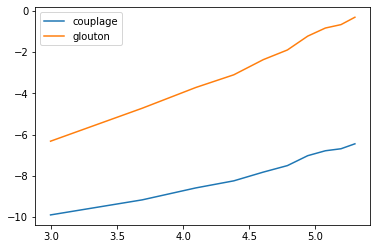
\includegraphics[scale=0.5]{figures/tps_exec_couglou25.png}
                    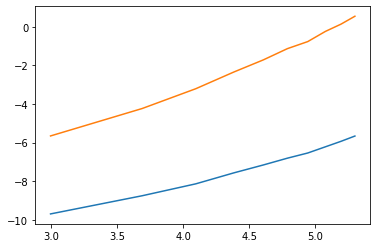
\includegraphics[scale=0.5]{figures/tps_exec_couglou5.png}
                    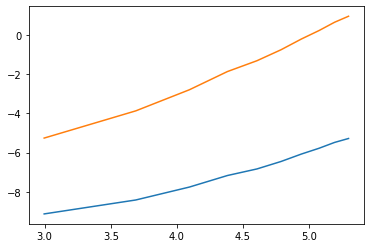
\includegraphics[scale=0.5]{figures/tps_exec_couglou75.png}
                    \centering
                \end{figure}

                Dans ces graphiques, nous pouvons observer que \texttt{algo\_couplage} est nettement meilleur que \texttt{algo\_glouton} en termes de temps d'exécution. \\
                Pour estimer la complexité de ces algorithmes, nous avons tracé la droite qui se rapproche le plus de nos données expérimentales (grâce à la fonction \texttt{polyfit} de \texttt{numpy}) pour mesurer sa pente. Par exemple, pour $p=0.25$, nous avons :
                
                \begin{figure}[H]
                    \centering
                    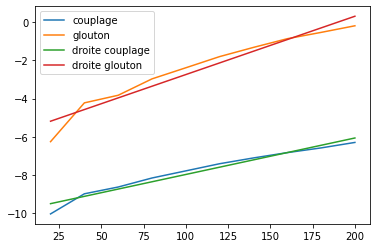
\includegraphics[scale=0.6]{figures/tps_exec_couglou25_droites.png}
                \end{figure}
                
                Nous avons comme pente 1.55 pour l'algorithme de couplage et 2.66 pour l'algorithme glouton. Ceci signifie que \texttt{algo\_couplage} est de complexité $O(n^{1.55})$ et \texttt{algo\_glouton} est de complexité $O(n^{2.66})$. On a donc bien que \texttt{algo\_couplage} est plus rapide que \texttt{algo\_glouton}.

            \item \textit{Comparaison du point de vue de la qualité de la solution} :  

                Le facteur principal pour évaluer la qualité des solutions est la dimension (i.e. la longueur) de la couverture. Nous allons donc comparer la dimension des solutions retournées par les deux algorithmes. \\
                Pour faire les tests, nous avons ici pris la moyenne sur 3 essais pour 30 valeurs de $n$ différentes jusqu'à 100.

                \paragraph{$p = 1$} 
                    Avec des graphes complets, nous trouvons des résultats très proches entre les deux méthodes : en effet, le rapport est $\dfrac{dim_{glouton}}{dim_{couplage}} = 0.993 $

                    %Nous sommes en-dessous d'une différence de 5\%, donc on peut supposer de préferer dans ce cas la methode mieux approchée ou plus rapide, selon les nécessités.

                    \begin{figure}[h]
                        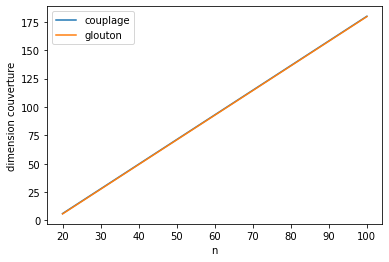
\includegraphics[scale=0.5]{figures/qualite_1.png}
                        \centering
                    \end{figure}

                    Nous pouvons en effet remarquer que \texttt{algo\_couplage} renvoie toujours comme couverture l'ensemble de tous les sommets (donc de taille $n$), puisque l'on ajoute les sommets deux par deux ; et \texttt{algo\_glouton} renvoie toujours une couverture de taille $n-1$ (qui est bien sûr une solution optimale).

                \paragraph{$p = 0.25$}
                    Nous observons que même en réduisant $p$ jusqu'à $0.25$, les résultats ne varient beaucoup non plus (nous avons effectué les tests pour les autres $p$, mais nous les excluons de ce document car ils n'apportent pas d'informations particulières).
                    
                    En effet, $\dfrac{dim_{glouton}}{dim_{couplage}} = 0.938 $, la différence entre les deux algorithmes est donc petite.
                    
                    \begin{figure}[H]
                        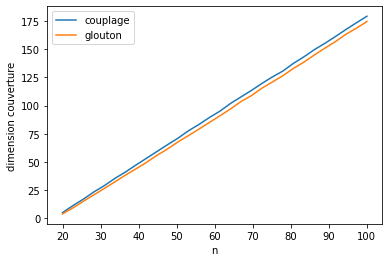
\includegraphics[scale=0.5]{figures/qualite_025.png}
                        \centering
                    \end{figure}
                
                \paragraph{$p = 1/ \sqrt{n}$}
                    Ce n'est qu'avec des graphes particulièrement vides que l'on commence à observer une différence de qualité remarquable.

                    En effet, $\dfrac{dim_{glouton}}{dim_{couplage}} = 0.858 $.
                    La méthode glouton prend le dessus ici, ce qui nous indique qu'avec des graphes de plus en plus vides, on s'approche des cas limites de l'algorithme de couplage.

                    \begin{figure}[H]
                        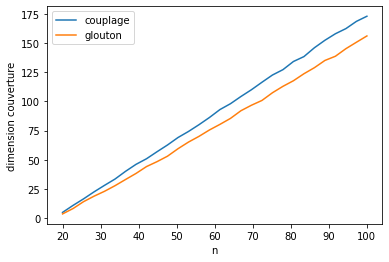
\includegraphics[scale=0.5]{figures/qualite_p.png}
                        \centering
                    \end{figure}

                Avec p qui varie de 0 à 1, on obtient le tableau suivant pour $\dfrac{dim_{glouton}}{dim_{couplage}}$ :

                \begin{center}
                    \begin{tabular}{ |c c c c c| } 
                    \hline
                    0.65384615 & 0.6875 &    0.70945946  & 0.71604938 & 0.74712644  \\
                    0.78888889 & 0.80337079 & 0.79891304 & 0.81914894 & 0.84375   \\
                    0.84210526  & 0.87894737 & 0.8814433 & 0.84848485 & 0.89175258 \\
                    0.88383838 &  0.91752577 & 0.90909091 & 0.915   &    0.95\\
                    \hline
                    \end{tabular}
                \end{center}

                Nous concluons en affirmant que l'algorithme glouton se révele meilleur en terme de qualité malgré un temps d'exécution plus long.
                Lorsqu'il y a beaucoup d'arêtes, la différence peut être considérée négligeable, mais avec des graphes ``vides", l'algorithme glouton prend un avantage plutôt fort.

        \end{enumerate}

\section{Méthodes exactes : algorithme de branch-and-bound}

    \paragraph{4.1.2)}
        La méthode décrite dans cette question correspond à notre fonction \texttt{branch}. \\
        La pile contient les nœuds de l'arbre à explorer. Chaque nœud est un couple $(G,C)$ où $G$ est le graphe réduit au fur et à mesure et $C$ la couverture en construction. \\
        Vérifions sa validité sur un exemple simple. Soit le graphe $J$ suivant :

        \begin{figure}[H]
            \caption{Graphe J}
            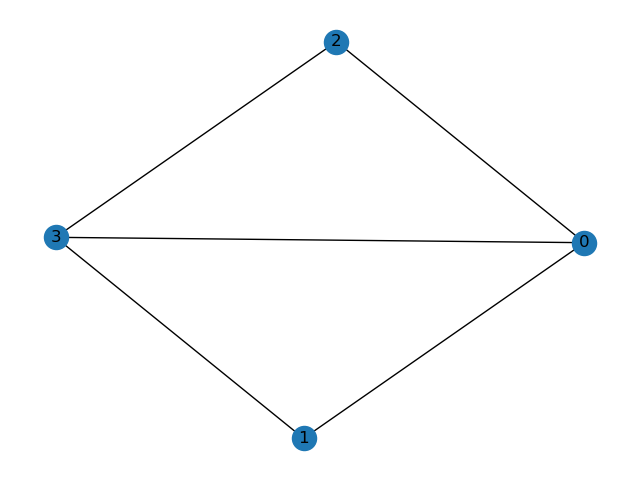
\includegraphics[scale=0.5]{figures/Figure_1.png}
            \centering
        \end{figure}

        Voici l'abre d'énumération de \texttt{branch} sur le graphe $J$. Dans chaque nœud, on choisit une arête, et on branche sur les extrémités de cette arête (le chiffre sur les arcs correspond au sommet choisi) :

        \begin{figure}[H]
            \caption{Arbre d'énumération pour l'instance J}
            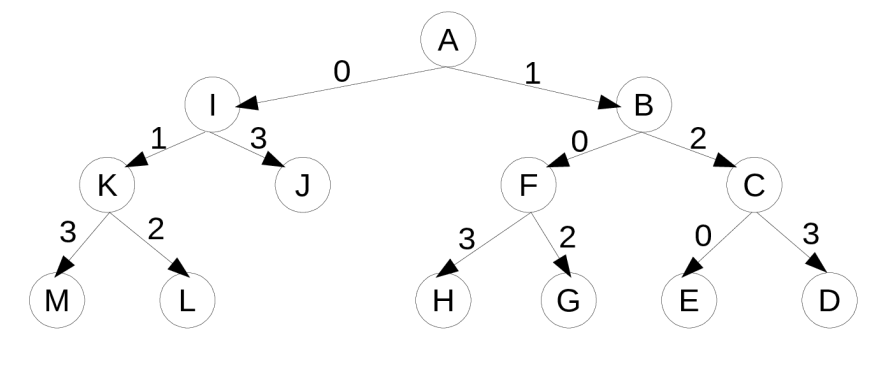
\includegraphics[scale=0.4]{figures/arbre_enum.png}
            \centering
        \end{figure}

        La description de chacun des nœuds est donné ci-dessous :

        \begin{itemize}
            \item A : $C_{tmp} = \{\}$ ; $G_{tmp}.edges=\{\{0,1\},\{1,3\},\{3,2\},\{0,2\},\{0,3\}\}$ ; arête choisie : \{0,1\}
            \item B : $C_{tmp} = \{1\}$ ; $G_{tmp}.edges=\{\{3,2\},\{0,2\},\{0,3\}\}$ ; arête choisie : \{0,2\}
            \item C : $C_{tmp} = \{1,2\}$ ; $G_{tmp}.edges=\{\{0,3\}\}$ ; arête choisie : \{0,3\}
            \item D : $C_{tmp} = \{1,2,3\}$ ; $G_{tmp}.edges=\{\}$
            \item E : $C_{tmp} = \{1,2,0\}$ ; $G_{tmp}.edges=\{\}$
            \item F : $C_{tmp} = \{1,0\}$ ; $G_{tmp}.edges=\{\{3,2\}\}$ ; arête choisie : \{3,2\}
            \item G : $C_{tmp} = \{1,0,2\}$ ; $G_{tmp}.edges=\{\}$
            \item H : $C_{tmp} = \{1,0,3\}$ ; $G_{tmp}.edges=\{\}$
            \item I : $C_{tmp} = \{0\}$ ; $G_{tmp}.edges=\{\{1,3\},\{3,2\}\}$ ; arête choisie : \{1,3\}
            \item J : $C_{tmp} = \{0,3\}$ ; $G_{tmp}.edges=\{\}$
            \item K : $C_{tmp} = \{0,1\}$ ; $G_{tmp}.edges=\{\{3,2\}\}$ ; arête choisie : \{3,2\}
            \item L : $C_{tmp} = \{0,1,2\}$ ; $G_{tmp}.edges=\{\}$
            \item M : $C_{tmp} = \{0,1,3\}$ ; $G_{tmp}.edges=\{\}$
        \end{itemize}

        Ainsi à la fin, on retourne \{0,3\} qui est bien la meilleure solution calculée.

    \paragraph{4.2.1)}
        Soit $G=(V,E)$ un graphe non orienté, où $V$ est l'ensemble des sommets et $E$ l'ensemble des arêtes. On note $n = |V|$ et $m = |E|$. \\
        Soit $M$ un couplage et $C$ une couverture de $G$. \\
        Posons $b_1 = \lceil \frac{m}{\Delta} \rceil$, $b_2 = |M|$ et $b_3 = \frac{2n-1 - \sqrt{(2n-1)^2 - 8m}}{2}$. \\
        Montrons que $|C| \geq b_1,b_2,b_3$.

        \begin{itemize}
            \item Soit $\Delta$ le degré maximum des sommets de $G$. Comme chaque sommet de $C$ est une extrémité d'au plus $\Delta$ arêtes, on a : $|C| \times \Delta \geq m \implies |C| \geq \frac{m}{\Delta}$. \\
            $|C|$ étant un entier, on peut prendre $b_1 = \lceil \frac{m}{\Delta} \rceil$ comme borne inférieure, d'où $\boxed{|C| \geq b_1}$. 
            
            \item Pour toute arête de $M$, une de ses extrémités est dans $C$ (sinon elle ne serait pas couverte et $C$ ne serait pas une couverture). De plus, ces extrémités sont toutes distinctes par définition d'un couplage. Ainsi on a bien $\boxed{|C| \geq b_2}$
            
            \item On souhaite déterminer le nombre maximal d'arêtes d'un graphe à $n$ sommets et de couverture $C$. Posons $|C| = x$. \\
            Dans le graphe, il y a deux types d'arêtes :
            \begin{itemize}
                \item celles dont les deux extrémités sont dans $C$ : il y a en a au plus $\frac{x(x-1)}{2}$ (c'est le nombre d'arêtes dans un graphe complet à $x$ sommets) car chaque sommet de $C$ est relié aux $x-1$ autres sommets de $C$, et on divise par 2 pour ne pas compter deux fois la même arête
                \item celles dont seule une extrémité est dans $C$ : il y en a au plus $x(n-x)$ car chaque sommet de $C$ est relié aux $n-x$ autres sommets qui n'appartiennent pas à $C$.
            \end{itemize}
            Il n'y en a pas d'autre car sinon elle ne serait pas couverte par $C$, ce qui contredirait le fait que $C$ soit une couverture.
            Ainsi, nous avons l'inégalité suivante :
            \begin{align*}
                m &\leq \frac{x(x-1)}{2} + x(n-x) \\
                \iff m &\leq \frac{x^2 - x + 2nx - 2x^2}{2} \\
                \iff m &\leq \frac{-x^2 + (2n-1)x}{2} \\
                \iff 0 &\leq \frac{-x^2 +(2n-1)x - 2m}{2} \\
                \iff 0 &\geq x^2 -(2n-1)x + 2m \\
                \iff x &\geq \frac{2n-1 + \sqrt{(2n-1)^2 - 8m}}{2} = b_3 \text{ (racine du polynôme de second degré)}
            \end{align*}
            Nous avons donc bien $\boxed{|C| \geq b_3}$
        \end{itemize}

    \paragraph{4.2.2)}
        Il s'agit de notre fonction \texttt{branch2}. \\
        A chaque nœud, on calcule le max des bornes inférieures du graphe considéré et on explore les nœuds fils uniquement cette borne inférieure est plus petite que la borne supérieure. \\
        Lorsqu'il n'y a plus d'arête dans le graphe, on compare la couverture que l'on a construite avec celle que l'on possède déjà, et on garde la meilleure des deux.
    
    \paragraph{4.3.1)}
        Il s'agit de la fonction \texttt{branch3}.

    \paragraph{4.3.2)}
        Il s'agit de la fonction \texttt{branch32}.

    \paragraph{Comparaison des algorithmes de branch-and-bound)}
        branch v1 est l'algorithme où nous explorons l'arbre d'énumération intégralement, branch v2 est celui où nous ajoutons le calcul des bornes inférieures et branch v3 correspond à notre fonction branch3.

        \begin{itemize}
            \item \textit{Comparaison de branch v1 et branch v2} \\
                Ici, nous nous sommes limités à $N_{max} = 20$ ou 30, et nous avons calculé les temps d'exécution pour $p = 1/\sqrt{n}$. \\
                Nous avons passé les temps au log base $e$.
    
                \begin{figure}[H]
                    \caption{Comparaison de branch v1 et branch v2}
                    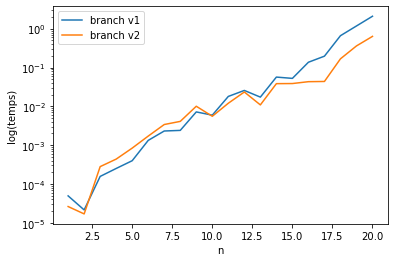
\includegraphics[scale=0.6]{figures/branch1-2_psqrt.png}
                    \centering
                \end{figure}
    
                Nous pouvons voir que quand $n$ est petit, branch v1 est meilleur, mais que pour des $n$ plus grands, branch v2 devient meilleur. \\
                Ceci peut s'expliquer par le fait que quand il y a peu de sommets et que $p$ est faible, parcourir l'arbre en entier ne prends pas autant de temps que de faire appel à la fonction \texttt{algo\_couplage}. En ravenche, plus $n$ est grand, plus l'arbre devient grand, et plus le calcul des bornes inférieures devient pertinent pour élaguer des nœuds.

            \item \textit{Comparaison de branch v2 et branch v2 avec l'algo glouton} \\
                \begin{figure}[h]
                    \caption{Comparaison de branch v2 et branch v2 glouton}
                    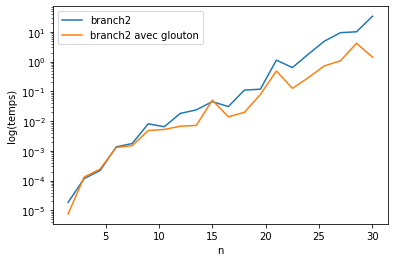
\includegraphics[scale=0.6]{figures/branch2-2glou.png}
                    \centering
                \end{figure}
                Nous observons que l'utilisation de l'algorthme glouton permet d'aller plus vite : comme il est de meilleure qualité, on peut élaguer plus de nœuds.

            \item \textit{Comparaison de branch v2 glouton et branch v3} \\
            \begin{figure}[h]
                \caption{Comparaison de branch v2 glouton et branch v3}
                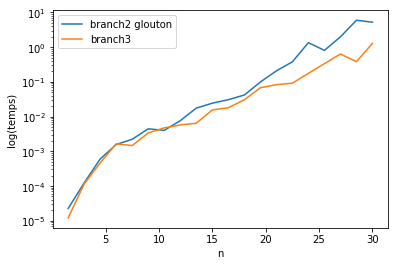
\includegraphics[scale=0.6]{figures/branch2glou-3.png}
                \centering
            \end{figure}
            Le branchement ayant été amélioré, branch v3 est plus rapide que branch v2 glouton.

            \item \textit{Comparaison de branch v3 et branch v3-2} \\
                branch v3-2 correspond à l'amélioration de branch v3 donnée dans la question 4.3.2 (dans notre code, il s'agit de la fonction \texttt{branch32}).
            \begin{figure}[H]
                \caption{Comparaison de branch v3 et branch v3-2}
                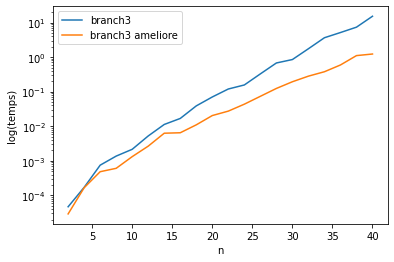
\includegraphics[scale=0.6]{figures/branch3-3amel.png}
                \centering
            \end{figure}
            De même, comme le branchement a été amélioré, le temps d'exécution de branch v3-2 est meilleur que le branch v3.
            
        \end{itemize}

    \paragraph{4.4.1)}
        Le graphique suivant montre l'évolution de la longueur de la couverture pour un graphe à $n=20$ sommets, en fonction de $p$.

        \begin{figure}[H]
            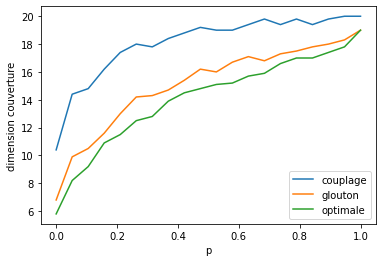
\includegraphics[scale=0.6]{figures/qualite_pvar.png}
            \centering
        \end{figure}

        On observe que plus il y a d'arêtes, plus la couverture est longue (ce qui est normal) et surtout que la longueur de la solution retournée par \texttt{algo\_glouton} est plus proche que celle d'\texttt{algo\_couplage} de la longueur de la solution optimale.
        
        On a en moyenne $\dfrac{dim_{glouton}}{dim_{optimale}} = 1.083 $ contre $\dfrac{dim_{couplage}}{dim_{optimale}} = 1.334 $. \\
        Ceci confirme que l'algorithme glouton donne une meilleure solution que l'algorithme de couplage puique son rapport d'approximation est plus petit.

\section{Conclusion générale}
    
    Les algorithmes approchés ont pour avantage de pouvoir tourner relativement rapidement sur des grands graphes, et la solution qu'ils retournent n'est pas particulièrement mauvaise. \\

    L'algorithme de branch-and-bound est plutôt efficace pour résoudre de manière exacte le problème du \textsc{vertex cover} et il peut toujours être amélioré grâces à des bonnes bornes inférieures et des bonnes heuristiques de branchement. Cela permet à la fois de gagner en temps d'exécution et de pouvoir calculer la couverture de graphes plus grands.       


\end{document}